\chapter{Análisis Teórico}
Se analizó el comportamento del circuito a pequeñas señales.
\section{Circuito de Polarización}
Como primer paso se analizó la polarización del circuito, ambos en su forma de carga pasiva (figura \ref{fig:pol_pasivo}) y activa (figura \ref{fig:pol_activo}).

\begin{figure} [ht]
    \centering
    \begin{minipage}{0.48\textwidth}
        \centering
        \begin{circuitikz}
            \ctikzset{resistors/scale=0.5};
            \draw
            (7,6.5) node[vcc](Vcc){$V_{CC}$}
            (5.5,5) node[npn](Q1){$Q_1$}
            (7,4) node[npn](Q2){$Q_2$}
            (Q1.E) |- (Q2.B)
            (Q1.C) |- (Vcc) (Q2.C) |- (Vcc)
            (Q1.B) to[R=$R_B$] ++(0,1.5) --(Vcc)
            (Q2.E) to[R=$R_E$] ++(0,-1) node[ground]{}
            ;
        \end{circuitikz}
        \caption{Circuito de Polarización con Carga Pasiva}
        \label{fig:pol_pasivo}
    \end{minipage}\hfill
    \begin{minipage}{0.48\textwidth}
        \centering
        \begin{circuitikz}
            \ctikzset{resistors/scale=0.5};
            \draw
            (7,6.5) node[vcc](Vcc){$V_{CC}$}
            (5.5,5) node[npn](Q1){$Q_1$}
            (7,4) node[npn](Q2){$Q_2$}
            (Q1.E) |- (Q2.B)
            (Q1.C) |- (Vcc) (Q2.C) |- (Vcc)
            (Q1.B) to[R=$R_B$] ++(0,1.5) --(Vcc)
            (Q2.E) to[I, l=$I_{ref}$] ++(0,-1) node[ground]{}
            ;
        \end{circuitikz}
        \caption{Circuito de Polarización con Carga Activa}
        \label{fig:pol_activo}
    \end{minipage}
\end{figure}

\subsection{Carga Pasiva}
En el circuito con Carga Pasiva, se resolvió analizando las mallas de entrada de los transistores.

\begin{align*}
    & V_{CC}-I_{B1}R_{B}-V_{BEon1}-V_{BEon2}-I_{E2}R_{E}=0 \\
    & I_{E2} = \left(1 + h_{FE1}\right)\left(1 + h_{FE2}\right) I_{B1} \\
    \Rightarrow & I_{E2} = \frac{V_{CC}-V_{BEon1}-V_{BEon2}}{R_E+\frac{R_B}{\left(1 + h_{FE1}\right)\left(1 + h_{FE2}\right)}}
\end{align*}

Considerando que la influencia de de $R_B$ será despreciable frente a la de $R_E$, y que ambos transistores tienen la misma $V_{BEon}$ se puede aproximar \eqref{eq:pol_I_E2}. Luego se pueden obtener las $I_{CQ}$ de cada transistor.

\begin{equation}
    I_{E2} \approx \frac{V_{CC}-2V_{BEon}}{R_E}
    \label{eq:pol_I_E2}
\end{equation}

\begin{align}
    I_{CQ2} &= \frac{h_{FE2}}{h_{FE2}+1}\cdot I_{E2} \label{eq:icq2} \\ 
    I_{CQ1} &= \frac{h_{FE1}}{h_{FE1}+1}\cdot \frac{1}{h_{FE2}+1}\cdot I_{E2} \label{eq:icq1}
\end{align}

Recorriendo las mallas de salida se obtuvieron las $V_{CEQ}$ de cada transistor.

\begin{align}
    V_{CEQ2} &= V_{CC} - I_{E2} R_E \\
    V_{CEQ1} &= V_{CC} - V_{BEon} - I_{E2} R_E
\end{align}

\subsection{Carga Activa}

A partir de la ecuación de Sah \eqref{eq:sah} para cada uno de los transistores se puede encontrar la razón entre la corriente de salida y de referencia.
\begin{equation}
    I_D = K' \frac{W}{L}\cdot (V_{GS}-V_{TH})^2
    \label{eq:sah}
\end{equation}

Considerando que por la configuración la tensión $V_{GS}$ será la misma para ambos transistores, y aproximando que, dado que se utilizarán transistores del mismo modelo, se puede aproximar que 

\begin{equation}
    I_o = \frac{(W/L)_3}{(W/L)_4} \cdot I_{ref}
\end{equation}

Por otro lado, puede diseñarse la $I_{ref}$ recorriendo la malla de $Q_4$

\begin{equation}
    I_{ref}=\frac{V_{DD}-V_{GS}}{R_{ref}}
    \label{eq:I_ref}
\end{equation}

Luego, los resultados de \eqref{eq:I_ref} pueden utilizarse en \eqref{eq:pol_I_E2}, \eqref{eq:icq2} y \eqref{eq:icq1}.

También a partir de la ecuación	 \eqref{eq:sah} se puede obtener las tensiones de polarización:

\begin{align}
    V_{DS} &= \sqrt{\frac{I_D L}{K' W}} + V_{TH}\\
    V_{CEQ2} &= V_{CC} - V_{DS} \\
    V_{CEQ1} &= V_{CC} - V_{DS} - V_{BEon}
\end{align}

\section{Parámetros de Pequeña Señal}

Antes de analizar el modelo de pequeña señal del par Darlington en configuración de seguidor de emisor, es necesario encontrar los parámetros del modelo híbrido, dadas por las siguientes ecuaciones..
%% Estaba Giacoletto, pero es mas facil las cuentas con hibrido. Nose si afecta el cambio
\begin{align}
    hie = \frac{\beta V_T}{I_{C1}} \\
    hfe = \approx \beta \\
    \frac{1}{hoe_1} = \frac{V_{A}}{I_{CQ}} \\
\end{align}
De las cuales a partir de la polarizacion previamente calculada, se obtienen los siguientes valores.

\begin{table}
    \centering
    \begin{tabular}{|c|c|c|}
     & $Q_1$ & $Q_2$ \\
    $hie$           &    &     \\
    $hfe$           &    &      \\
    $\frac{1}{hoe}$ &    &      \\
    \end{tabular}
\end{table}


%%  MEJORAR IMPEDANCIA DE SALIDA DE FUENTE DE CORRIENTE

A su vez es necesario calcular la impedencia de salida de la fuente de corriente. Al ser esta la carga activa, su impedancia de salida es la que vera el par Darlington en reemplazo de la resistencia $R_E$.
Ya que es aqui especificamente donde se ve la mejora al circuito basico, es primordial tener un valor numerico para resaltarla. Como se trata de una fuente espejo con MOS-FET, se estima la impedancia de salida con la expresion de la ecuacion \ref{eq:imp salida fte corriente}.
\begin{equation}
    R_O = \frac{V_A}{I_0} 
    \label{eq:imp salida fte corriente}
\end{equation}
Dada la polariacion especificada, se haya valor numerico para $R_O =XX \Omega$.

\section{Circuito Incremental}

Se reemplazan los transistores bipolares por su modelo híbrido para la pequeña señal en las figuras \ref{fig:circuito_pasivo} y \ref{fig:circuito}. Para esta ultima se considera la impedancia de salida ($R_O$) de la fuente espejo, en vez de la resistencia $R_E$.
Se llega de esta manera en el circuito incremental pertinente, ilustrado en la figura \ref{fig:circuito incremental darlington}.

\begin{figure}[ht]
    \centering
    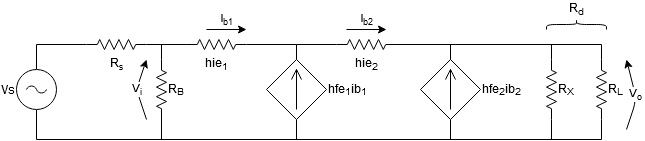
\includegraphics[scale=0.5]{2_teorico/figs/Incremental Darlington.png}
    \caption{Circuito Incremental}
    \label{fig:circuito incremental darlington}
\end{figure}
En donde $R_X$ dependiendo del análisis se considera $R_E$ con carga pasiva y $R_O$ con carga activa. 


\subsection{Impedancia Entrada}

La expresion para la impedancia de entrada se obtiene a traves de un pasaje de corriente, al considerarse $i_{b2} = (1+hfe_1)i_{b1}$.
\begin{equation}
    R_i = hie_1 + (1+hfe_1)hie_2 + (1+hfe_1)(1+hfe_2)R_D
    \label{eq:Impedancia de entrada}
\end{equation}

\subsection{Ganancia de Tensión}
A partir de la ecuacion \ref{eq:Impedancia de entrada}, se desarrolla la ganancia $\Delta_V$.
\begin{align}
    \Delta_V = \frac{V_o}{V_i} = \frac{V_o}{i_{b2}} \frac{i_{b2}}{i_{b1}} \frac{i_{b1}}{V_i} \\
    \Delta_V = \frac{R_D(1+hfe_1)(1+hfe_2)}{R_D(1+hfe_1)(1+hfe_2) + hie_1 + hie_2(1+hfe_2)}
\end{align}
Sacando factor comun se obtiene:
\begin{equation}
    \Delta_V = \frac{1}{\frac{hie_1 + hie_2(1+hfe_2)}{R_D(1+hfe_1)(1+hfe_2)}{R_D(1+hfe_1)(1+hfe_2)}}
\end{equation}
Como se tiene que la ganancia ideal de un seguidor de emisor es $\Delta_V \approx 1$...


\subsection{Ganancia de Corriente}
Lorem ipsum
\subsection{Impedancia de Salida}
Lorem ipsum
\subsection{Respuesta en Frecuencia}
Lorem ipsum

\section{Selección de Componentes}
\subsection{Limitaciones de la Plataforma de Medición} \label{sec:EE_limits}

Dado que el \textit{Electronics Explorer} sobre el cual se hicieron las mediciones tiene un límite de corriente de $1.5 \si{\ampere}$ en las salidas programables, se diseñaron los circuitos de forma de no saturar al dispositivo. La salida $V_{cc}$ no tiene limitación de corriente, pero la tensión es muy baja.

Como se planea utilizar un espejo de corriente, donde se consideró que ambos transistores n-mos son idénticos, las corrientes de polarización que se le pedirán a la fuente estarán dadas por:

\begin{align*}
    I_{CQ} &= \frac{h_{fe}}{h_{fe}+1} \cdot I_{EQ} \\
    I_{BQ} &= \frac{1}{h_{fe}+1} \cdot I_{EQ}\\
    I_{CQ2} &= I_o = I_{ref} \\
    I &= I_{ref} + I_{CQ2} + I_{CQ1} + I_{BQ1}
\end{align*}

\begin{equation}
    \Rightarrow I = I_{ref} \left(1 + \frac{h_{fe2}}{h_{fe2}+1} + \frac{1}{h_{fe2}+1}\cdot\frac{h_{fe1}}{h_{fe1}+1}+\frac{1}{h_{fe2}+1}\cdot\frac{1}{h_{fe1}+1}\right)
\end{equation}

Aproximando a valores altos de ganancias de corriente,

\begin{equation}
    I \approx I_{ref}\left(2+1/h_{fe2}\right)
\end{equation}

A partir de la expresión anterior se consideró entonces una cota máxima de la corriente de referencia:
\begin{equation}
    I_{ref} < 0.75 \si{\ampere}
    \label{eq:Iref}
\end{equation}

\section{Comparacion Teorica Carga activa y pasiva}

%%Nose donde ponerlo, pero estimo que debe ir en esta seccion. Es mostrar como con la RO se obtiene mejor AV
%% Y la relacion de compromiso con RE(corriente y ganancia), lo que dijo en clase.